\subsection{准希尔伯特空间的凸子集}

若对准希尔伯特空间 E 的任意两点 x, y 计算 \(\|x - y\|^{2} = \langle x - y|x - y \rangle\) 与 \(\|x + y\|^{2} = \langle x + y|x + y \rangle\) ，立即得到«中线恒等式»

\[
\left\| \frac {1}{2} (x + y) \right\| ^ {2} + \left\| \frac {1}{2} (x - y) \right\| ^ {2} = \frac {1}{2} (\| x \| ^ {2} + \| y \| ^ {2}).\tag{14}
\]

由这个恒等式我们导出下列命题：

\pandocbounded{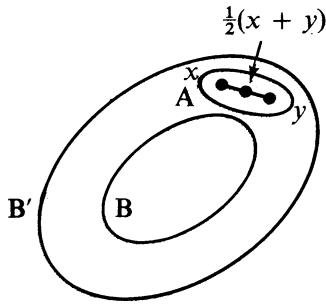
\includegraphics[keepaspectratio]{images/part002_56de9e6b.jpg}}\\
图 1.

命题 5. --- 设 E 为准希尔伯特空间。设 d 为实数 \textgreater0，δ 为使 \(0 \leqslant \delta \leqslant d\) 的实数。设 B 与 B' 为 E 的子集，分别由 \(\|x\| < d\) 与 \(\| x\| \leqslant d + \delta\) 定义，并设 A 为含于 \(\mathbf{B}' - \mathbf{B}\) 的凸集。则对 A 的每对点 \(x, y\) ，有 \(\| x - y\| \leqslant \sqrt{12d\delta}\) （图~1）。

事实上，我们有 \(\frac{1}{2} (x + y)\in \mathbf{A}\) ，故 \(\| \frac{1}{2} (x + y)\| \geqslant d\) ；于是由 (14) 得不等式

\[
\left\| \frac {1}{2} (x - y) \right\| ^ {2} = \frac {1}{2} \left(\| x \| ^ {2} + \| y \| ^ {2}\right) - \left\| \frac {1}{2} (x + y) \right\| ^ {2} \leqslant (d + \delta) ^ {2} - d ^ {2} \leqslant 3 d \delta
\]

由此即得命题。

定理 1. --- 设 E 为准希尔伯特空间，H 为 E 的一个非空凸子集，使得 H 是 E 的 Hausdorff 且完备的一致子空间。对每个 \(x \in E\) ，在 H 中存在唯一的点 \(p_{\mathrm{H}}(x)\) 使 \(\|x - p_{\mathrm{H}}(x)\| = \inf_{y \in \mathrm{H}} \|x - y\|\) 。H 的元素 \(p_{\mathrm{H}}(x)\) 也是 H 中满足关系式 \(^{1}\) 的唯一元素 a

\[
\mathcal {R} \langle x - a | y - a \rangle \leqslant 0\tag{15}
\]

对所有 \(y \in \mathbf{H}\) 成立。

\pandocbounded{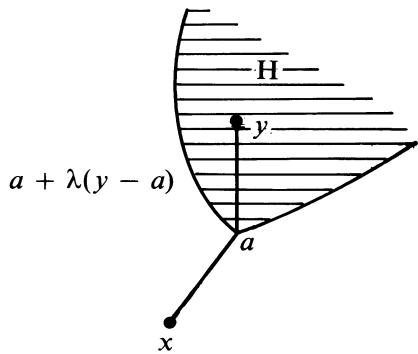
\includegraphics[keepaspectratio]{images/part002_6909685c.jpg}}\\
图 2.

令 \(d = \inf_{y \in \mathbf{H}} \| x - y \|\) ，且对每个整数 \(n > 0\) ，设 \(\mathrm{H}_n\) 为点 \(y\) （在 \(\mathbf{H}\) 中，使 \(\| x - y \| \leqslant d + n^{-1}\) ）所成的集。集 \(\mathrm{H}_n\) 在 \(\mathbf{H}\) 中是闭的，是凸的且非空，且由命题 5，其直径以 \(\sqrt{12d / n}\) 为界（对所有足够大的 \(n\) ）。由于序列 \((\mathrm{H}_n)_{n \geqslant 1}\) 递减，且集 \(\mathbf{H}\) 是 Hausdorff 且完备的，因此 Cauchy 滤子 \((\mathrm{H}_n)_{n \geqslant 1}\) 的基收敛到一点 \(p_{\mathbf{H}}(x)\) （属于 \(\mathbf{H}\) ）；我们有 \(\{p_{\mathbf{H}}(x)\} = \bigcap_{n \geqslant 1} \mathrm{H}_n\) ，故 \(p_{\mathbf{H}}(x)\) 是唯一的点 \(a\) （在 \(\mathbf{H}\) 中），使 \(\| x - a \| = d\) 。

\(^{1}\) 我们回顾（GT, VIII, § 1, No.~1），\(\mathcal{R}(z)\) 表示复数 z 的实部；若 z 是实数，则有 \(\mathcal{R}(z)=z\) 。

设 \(y \in H\) ；由于 \(H\) 是凸的，点 \(z(\lambda) = p_{\mathbf{H}}(x) + \lambda(y - p_{\mathbf{H}}(x))\) （\(E\) 中的）属于 \(H\) ，对每个实数 \(\lambda\) （满足 \(0 < \lambda < 1\) 的）。因此我们有

\[
\left\| x - z (\lambda) \right\| ^ {2} \geqslant \left\| x - p _ {\mathrm{H}} (x) \right\| ^ {2} \quad \text { for } \quad 0 <   \lambda <   1,
\]

由此给出

\[
\mathcal {R} \left\langle x - p _ {\mathrm{H}} (x) \mid y - p _ {\mathrm{H}} (x) \right\rangle = \lim _ {\lambda \rightarrow 0} \frac {1}{2 \lambda} \left\{\| x - p _ {\mathrm{H}} (x) \| ^ {2} - \| x - z (\lambda) \| ^ {2} \right\} \leqslant 0.
\]

反之，设 \(a\) 为 \(\mathbf{H}\) 的一点，使 \(\mathcal{R}\langle x - a|y - a\rangle \leqslant 0\) 对所有 \(y\in \mathbf{H}\) 成立。对每个 \(y\in \mathbf{H}\) ，有

\[
\left\| x - y \right\| ^ {2} = \left\| x - a \right\| ^ {2} + \left\| y - a \right\| ^ {2} - 2 \mathcal {R} \langle x - a | y - a \rangle \geqslant \left\| x - a \right\| ^ {2},
\]

于是 \(\| x - a\| = d\) ，最后由证明的第一部分得出 \(a = p_{\mathrm{H}}(x)\) 。证毕。

在下面，E 到 H 中的映射 \(p_{H}\) 将称为从 E 到 H 上的投影。我们注意 \(p_{\mathrm{H}}(x)=x\) 对所有 \(x\in H\) 成立。

定理 1 的第一部分在关于空间 E 的更一般假设下仍然成立（V, p.~67, 练习 31）。

定理 1 的证明特别建立了下列性质：

推论 1. --- 设 I 为被滤子 \(\mathfrak{F}\) 定向的集合，\((y_i)_{i\in I}\) 为 H 的点的一个族。设 \(x\in E\) 。假设我们有

\[
\lim _ {i, \mathfrak {F}} \| x - y _ {i} \| = \inf _ {z \in \mathrm{H}} \| x - z \|.
\]

则 \(y_{i}\) 趋于 \(p_{\mathrm{H}}(x)\) （关于滤子 \(\mathfrak{F}\) ）。

推论 2. --- 对 E 中每个 x, y，有

\[
\left\| p _ {\mathrm{H}} (x) - p _ {\mathrm{H}} (y) \right\| \leqslant \left\| x - y \right\|.
\]

特别地，从 E 到 H 中的映射 \(p_{H}\) 是连续的。

设 \(x, y\) 为 \(E\) 的两点。令 \(a = p_{\mathrm{H}}(x) - x\) ，\(b = p_{\mathrm{H}}(y) - p_{\mathrm{H}}(x)\) ，\(c = y - p_{\mathrm{H}}(y)\) 。由公式 (15)（V, p.~10）我们有 \(\mathcal{R}\langle a|b\rangle \geqslant 0\) 与 \(\mathcal{R}\langle c|b\rangle \geqslant 0\) 。我们还有 \(a + b + c = y - x\) ，由此给出

\[
\| x - y \| ^ {2} = \| a + b + c \| ^ {2} = \| b \| ^ {2} + \| a + c \| ^ {2} + 2 \mathscr {R} \langle a | b \rangle + 2 \mathscr {R} \langle c | b \rangle
\]

\[
\geqslant \| b \| ^ {2} = \left\| p _ {\mathrm{H}} (x) - p _ {\mathrm{H}} (y) \right\| ^ {2}.
\]

这就证明了推论 2。

命题 6. --- 设 E 为准希尔伯特空间，\(\Phi\) 为由 E 的非空、Hausdorff 且完备的凸子集组成的非空递减有向集。对每个 \(x \in \mathrm{E}\) 与 E 的每个子集 H，令 \(d(x, \mathrm{H}) = \inf_{z \in \mathrm{H}} \| x - z \|\) 。为使属于 \(\Phi\) 的诸集 H 的交 M 非空，必要且充分的是存在 E 中的 \(x_0\) 使 \(\sup_{\mathbf{H} \in \Phi} d(x_0, \mathbf{H})\) 有限。这时对每个 \(x \in \mathbf{E}\) 我们有

\(p_{\mathbf{M}}(x) = \lim_{\mathrm{H}\in \Phi}p_{\mathrm{H}}(x)\) （关于有向集 \(\Phi\) 的极限）。

若 \(\mathbf{M}\) 非空，则 \(d(x,\mathrm{H})\leqslant d(x,\mathbf{M})\) 对所有 \(\mathbf{H}\in \Phi\) 与所有 \(x\in \mathbb{E}\) 成立。

反之，假设存在一点 \(x_0\) （在 \(\mathbf{E}\) 中）与实数 \(\mathbf{C} \geqslant 0\) ，使 \(d(x_0, \mathbf{H}) \leqslant \mathbf{C}\) 对所有 \(\mathbf{H} \in \Phi\) 成立。设 \(x \in \mathbf{E}\) ；则

\[
d (x, \mathrm{H}) \leqslant \| x - x _ {0} \| + \mathrm{C} \quad \text { for   all } \quad \mathrm{H} \in \Phi ,
\]

于是数 \(d = \sup_{\mathbf{H} \in \Phi} d(x, \mathbf{H})\) 有限。设 \(\mathbf{B}\) 为全体 \(z \in E\) （使 \(\| x - z\| \leqslant d\) 的）组成的集。由于 \(\mathbf{B}\) 在 \(\mathbf{E}\) 中是凸的且闭的，故诸集 \(\mathrm{H} \cap \mathrm{B}\) （当 \(\mathrm{H}\) 取遍 \(\Phi\) ）是凸的、Hausdorff 的且完备的。设 \(\varepsilon > 0\) ；存在集 \(\mathrm{H} \in \Phi\) 使 \(d(x, \mathrm{H}) \geqslant \mathrm{d} - \varepsilon\) ，且若 \(\varepsilon < d/2\) ，则 \(\mathrm{H} \cap \mathrm{B}\) 的直径由命题 5（V, p.~9）以 \(\sqrt{12\varepsilon(d - \varepsilon)}\) 为界。换言之，对所有 \(\mathrm{H}_0 \in \Phi\) ，诸闭集 \(\mathrm{H} \cap \mathrm{B}\) （\(\mathrm{H} \in \Phi\) 且 \(\mathrm{H} \subset \mathrm{H}_0\) ）构成 Hausdorff 完备空间 \(\mathrm{H}_0\) 上 Cauchy 滤子的一个基。因此诸集 \(\mathrm{H} \cap \mathrm{B}\) （对 \(\mathrm{H} \in \Phi\) ）的交化为一点 \(y\) 。我们得到 \(y \in \mathbf{M}\) 与 \(\| x - y \| = d = d(x, \mathbf{M})\) 。由于 \(\mathbf{M}\) 在 \(\mathrm{H}_0\) 中是闭的，它是 \(\mathbf{E}\) 中 Hausdorff、凸且完备的集，故 \(y = p_{\mathbf{M}}(x)\) 。对每个 \(\mathrm{H} \in \Phi\) ，我们有 \(p_{\mathrm{H}}(x) \in \mathrm{H} \cap \mathrm{B}\) ，由此得出 \(p_{\mathbf{M}}(x) = \lim_{\mathrm{H} \in \Phi} p_{\mathrm{H}}(x)\) 。

命题 7. --- 设 E 为 Hausdorff 准希尔伯特空间，\(\Psi\) 为由 E 的非空、凸、完备子集组成的非空递增有向集。令 \(A = \bigcup_{H \in \Psi} H\)

并假设闭包 \(\mathbf{N}\) （\(\mathbf{A}\) 的）是完备的。则 \(\mathbf{N}\) 是凸的，且 \(p_{\mathrm{N}}(x) = \lim_{\mathrm{H}\in \Psi}p_{\mathrm{H}}(x)\) 对所有 \(x\in \mathrm{E}\) 成立。

显然 A 是凸的，故其闭包 N 是凸的（II, p.~13）。采用命题 6 的记号，\(d(x, \mathrm{N}) = \inf_{\mathrm{H} \in \Psi} d(x, \mathrm{H})\) ，因此 \(d(x, \mathrm{N})\) 是 \(d(x, \mathrm{H})\) 关于 \(\Psi\) 的截面滤子的极限。由于 \(p_{\mathrm{H}}(x) \in \mathrm{H}\) 且

\[
\lim _ {\mathrm{H} \in \Psi} \| x - p _ {\mathrm{H}} (x) \| = \lim _ {\mathrm{H} \in \Psi} d (x, \mathrm{H}) = d (x, \mathrm{N}),
\]

由 V, p.~11 的推论 1 得出，\(p_{\mathrm{H}}(x)\) 趋于投影 \(p_{\mathrm{N}}(x)\) （\(x\) 到 \(\mathbf{N}\) 上的），这是关于 \(\Psi\) 的截面滤子而言的。

